\documentclass[12pt,a4paper]{article}

% ─── Page Layout ───────────────────────────────────────────────────────────────
\usepackage[a4paper, margin=0.8in, headheight=14pt]{geometry}

% ─── Fonts (XeLaTeX) ───────────────────────────────────────────────────────────
\usepackage{fontspec}
\usepackage{unicode-math}
\setmainfont{TeX Gyre Pagella}
\setmonofont[Scale=0.88]{TeX Gyre Cursor}
\setmathfont{Latin Modern Math}

% ─── Packages ──────────────────────────────────────────────────────────────────
\usepackage{xcolor}
\usepackage{colortbl}
\usepackage{titlesec}
\usepackage{enumitem}
\usepackage{tabularx}
\usepackage{booktabs}
\usepackage{array}
\usepackage{amsmath}
\usepackage{tikz}
\usetikzlibrary{shapes.geometric, arrows.meta, positioning, calc, fit, decorations.pathreplacing, patterns}
\usepackage{tcolorbox}
\tcbuselibrary{skins, breakable}
\usepackage{hyperref}
\usepackage{fancyhdr}
\usepackage{graphicx}
\usepackage{microtype}
\hyphenpenalty=10000
\exhyphenpenalty=10000
\sloppy
\usepackage{caption}
\usepackage{setspace}
\usepackage{multirow}
\usepackage{tocloft}

% ─── Q&A helper ────────────────────────────────────────────────────────────────
\newcommand{\Q}[1]{\textbf{#1}\par\noindent\ignorespaces}

% ─── Colour Palette ────────────────────────────────────────────────────────────
\definecolor{myred}{RGB}{196,30,58}
\definecolor{mydark}{RGB}{30,30,50}
\definecolor{mygreen}{RGB}{14,120,80}
\definecolor{myteal}{RGB}{0,130,140}
\definecolor{myamber}{RGB}{180,100,0}
\definecolor{mypurple}{RGB}{100,30,160}
\definecolor{mygray}{RGB}{246,247,249}
\definecolor{mgframe}{RGB}{180,185,200}
\definecolor{watermark}{RGB}{145,150,170}
\definecolor{hdrred}{RGB}{250,232,235}
\definecolor{hdrgreen}{RGB}{220,244,233}
\definecolor{hdrteal}{RGB}{220,242,244}
\definecolor{hdramber}{RGB}{253,242,215}
\definecolor{hdrpurple}{RGB}{238,228,255}
\definecolor{hdrgray}{RGB}{238,240,245}
\definecolor{rowalt}{RGB}{250,251,253}

% ─── Section Formatting ────────────────────────────────────────────────────────
\titleformat{\section}{\large\bfseries\color{myred}}{\thesection.}{0.5em}{}[\vspace{1pt}{\color{myred}\rule{\linewidth}{0.8pt}}]
\titleformat{\subsection}{\normalsize\bfseries\color{myteal}}{\thesubsection}{0.5em}{}
\titlespacing*{\section}{0pt}{18pt}{77pt}
\titlespacing*{\section}{0pt}{18pt}{7pt}
\titlespacing*{\subsection}{0pt}{11pt}{4pt}

% ─── Paragraph ─────────────────────────────────────────────────────────────────
\setlength{\parindent}{0pt}
\setlength{\parskip}{4pt}

% ─── TOC Styling ───────────────────────────────────────────────────────────────
\renewcommand{\cfttoctitlefont}{\large\bfseries\color{myred}}
\renewcommand{\cftaftertoctitle}{\par\noindent{\color{myred}\rule{\linewidth}{0.8pt}}}
\setlength{\cftbeforetoctitleskip}{0pt}
\setlength{\cftaftertoctitleskip}{6pt}
\renewcommand{\cftsecfont}{\normalsize\bfseries\color{mydark}}
\renewcommand{\cftsecpagefont}{\normalsize\bfseries\color{mydark}}
\renewcommand{\cftsecleader}{\cftdotfill{\cftdotsep}}
\setlength{\cftbeforesecskip}{7pt}
\renewcommand{\cftsubsecfont}{\small\color{mydark}}
\renewcommand{\cftsubsecpagefont}{\small\color{mydark}}
\setlength{\cftbeforesubsecskip}{3pt}
\setlength{\cftsubsecindent}{1.4em}

% ─── Table helpers ─────────────────────────────────────────────────────────────
\renewcommand{\arraystretch}{1.45}
\setlength{\tabcolsep}{6pt}
\arrayrulecolor{mydark}
\newcolumntype{B}[1]{>{\small\bfseries\raggedright\arraybackslash}m{#1}}
\newcolumntype{Y}{>{\small\raggedright\arraybackslash}X}
\renewcommand{\tabularxcolumn}[1]{m{#1}}

% ─── Header / Footer ───────────────────────────────────────────────────────────
\pagestyle{fancy}
\fancyhf{}
\fancyhead[L]{\small\color{myred}\textbf{OE-EC803A}\;\color{mydark}--- Internet of Things}
\fancyhead[R]{\small\color{myteal}\textbf{Module 3 Notes}}
\fancyfoot[C]{\small\color{mydark}\thepage}
\fancyfoot[R]{\small\color{watermark}\textit{\copyright\ Biraj Sarkar}}
\renewcommand{\headrulewidth}{0.5pt}
\renewcommand{\footrulewidth}{0.3pt}

% ─── Hyperref ──────────────────────────────────────────────────────────────────
\hypersetup{colorlinks=true, linkcolor=myteal, urlcolor=myteal,
  pdfauthor={Biraj Sarkar}, pdftitle={OE-EC803A --- Module 3 Notes}}

% ─── tcolorbox styles ──────────────────────────────────────────────────────────
\tcbset{
  tikzbox/.style={colback=mygray, colframe=mgframe, boxrule=0.6pt, arc=4pt,
    left=8pt, right=8pt, top=6pt, bottom=6pt,
    colbacktitle=mgframe, coltitle=mydark, fonttitle=\small\bfseries},
  defbox/.style={colback=hdrgreen, colframe=mygreen, boxrule=0.8pt, arc=4pt,
    left=9pt, right=9pt, top=6pt, bottom=6pt,
    colbacktitle=mygreen, coltitle=white, fonttitle=\small\bfseries},
  formulabox/.style={colback=hdrteal, colframe=myteal, boxrule=0.8pt, arc=4pt,
    left=9pt, right=9pt, top=7pt, bottom=7pt,
    colbacktitle=myteal, coltitle=white, fonttitle=\small\bfseries},
  examplebox/.style={colback=hdramber, colframe=myamber, boxrule=0.8pt, arc=4pt,
    left=9pt, right=9pt, top=6pt, bottom=6pt,
    colbacktitle=myamber, coltitle=white, fonttitle=\small\bfseries},
  masonbox/.style={colback=hdrpurple, colframe=mypurple, boxrule=0.8pt, arc=4pt,
    left=9pt, right=9pt, top=6pt, bottom=6pt,
    colbacktitle=mypurple, coltitle=white, fonttitle=\small\bfseries},
  exambox/.style={colback=hdrpurple, colframe=mypurple, boxrule=1pt, arc=5pt,
    left=10pt, right=10pt, top=8pt, bottom=8pt,
    colbacktitle=mypurple, coltitle=white, fonttitle=\bfseries,
    breakable, title after break={\textbf{Frequently Asked / Viva Questions (contd.)}}}
}
\tcbset{breakable}

% ─── TikZ styles ───────────────────────────────────────────────────────────────
\tikzset{
  block/.style={rectangle, draw=myteal, fill=hdrteal,
    text width=2.2cm, align=center, minimum height=0.85cm,
    font=\small, rounded corners=3pt, line width=0.7pt},
  arrow/.style={-Stealth, thick, color=mydark},
  line/.style={draw, thick, color=mydark}
}

\begin{document}

% ═══════════════════════════════════════════════════════════════════════════════
% TITLE BLOCK
% ═══════════════════════════════════════════════════════════════════════════════
\begin{center}
  \hfill \textit{Exam-Ready Short Notes} \\
  \vspace{6pt}
  {\LARGE\bfseries\color{myred} OE-EC803A --- Internet of Things}\\[5pt]
  {\normalsize\color{mydark} Semester VIII \quad$\bullet$\quad 3L:0T:0P \quad$\bullet$\quad 3 Credits}\\[3pt]
  {\normalsize\color{myteal}\textbf{Module 3: Prototyping: Thinking \& Embedded Hardware Platforms}}\\[3pt]
  {\small\color{mydark} CGEC \;$|$\; B.Tech ECE (2023--27) \;$|$\; \textit{Biraj Sarkar}}
\end{center}
\vspace{2pt}
\noindent{\color{myred}\rule{\linewidth}{1.5pt}}
\vspace{2pt}

\hypersetup{linkcolor=mydark}
\tableofcontents
\hypersetup{linkcolor=myteal}
\newpage

% ===============================================================================
\section{Thinking About Prototyping}
% ===============================================================================

Prototyping is the iterative process of quickly assembling a working model of a device to test assumptions and functionality before entering mass manufacturing.

\subsection{Prototyping Considerations}
\begin{itemize}[leftmargin=*, itemsep=3pt]
  \item \textbf{Sketching:} Fast, non-functional drawings to visualize hardware forms and user flows.
  \item \textbf{Familiarity:} Choosing tools the designer already knows (e.g. Arduino IDE) to reduce development time, even if other tools are mathematically more optimal.
  \item \textbf{Costs vs. Ease:} Fast prototyping tools (like jumper wires and breadboards) are cheap and easy, but produce bulky, fragile systems. Production-ready designs require custom PCBs.
  \item \textbf{Open Source vs. Closed Source:} Open hardware/software allows developers to adapt existing code libraries and hardware schematics, tapping into massive global communities.
\end{itemize}

% ===============================================================================
\section{Basic Electronics for IoT}
% ===============================================================================

IoT edge nodes interface directly with the physical world using sensors and actuators.

\subsection{Basic Quantities}
\begin{tcolorbox}[formulabox, title={Ohm's Law and Electrical Power}]
  \textbf{Ohm's Law} relates voltage ($V$), current ($I$), and resistance ($R$):
  \begin{equation}
    V = I \cdot R
  \end{equation}
  Electrical power ($P$) in watts is given by:
  \begin{equation}
    P = V \cdot I = I^2 \cdot R
  \end{equation}
\end{tcolorbox}

\begin{tcolorbox}[formulabox, title={Voltage Dividers and Analog-to-Digital Conversion (ADC)}]
  \textbf{Voltage Divider Formula:} Reduces a high analog voltage ($V_{\text{in}}$) to a safe range ($V_{\text{out}}$) for microcontroller pins:
  \begin{equation}
    V_{\text{out}} = V_{\text{in}} \cdot \left( \frac{R_2}{R_1 + R_2} \right)
  \end{equation}
  \textbf{ADC Resolution:} Quantizes an analog voltage into a digital integer. For an $n$-bit ADC with reference voltage $V_{\text{ref}}$, the step size (Resolution) is:
  \begin{equation}
    \text{Step Size (LSB)} = \frac{V_{\text{ref}}}{2^n}
  \end{equation}
  The measured digital value $D$ for an input voltage $V_{\text{in}}$ is:
  \begin{equation}
    D = \text{round}\left( \frac{V_{\text{in}}}{\text{Step Size}} \right) = \text{round}\left( V_{\text{in}} \cdot \frac{2^n}{V_{\text{ref}}} \right)
  \end{equation}
\end{tcolorbox}

\subsection{Signals and Interface Elements}
\begin{itemize}[leftmargin=*, itemsep=3.5pt]
  \item \textbf{Digital vs. Analog:} Digital signals are binary ($0$ or $1$, representing $0\text{V}$ and $3.3\text{V}/5\text{V}$). Analog signals vary continuously (e.g., LDR resistance changing with light).
  \item \textbf{PWM (Pulse Width Modulation):} Mimics analog outputs from a digital pin by switching the pin ON and OFF very rapidly. The ratio of ON time to the period is called the \textbf{Duty Cycle ($D$)}:
        \begin{equation}
          V_{\text{eff}} = D \cdot V_{\text{max}}
        \end{equation}
  \item \textbf{DHT11 Sensor:} A digital sensor measuring temperature and humidity, sending data over a single-wire digital protocol.
  \item \textbf{Relay:} An electromagnetic switch allowing a low-power microcontroller pin to switch high-voltage/high-current AC devices.
\end{itemize}

% ===============================================================================
\section{Prototyping Embedded Platforms}
% ===============================================================================

IoT designs select hardware platforms based on processing power, OS requirements, and connectivity.

\subsection{Embedded Computing Basics}
\begin{itemize}[leftmargin=*, itemsep=3pt]
  \item \textbf{Microcontroller (MCU):} A single integrated circuit containing a CPU, RAM, Flash memory, and I/O peripherals (GPIO, ADC, SPI, I2C). Low-power, real-time execution. Example: ATmega328P.
  \item \textbf{Microprocessor (MPU):} Contains only the CPU. Requires external RAM, Flash, and support ICs. Runs complex Operating Systems (Linux). High power consumption. Example: ARM Cortex-A72.
\end{itemize}

\begin{tcolorbox}[tikzbox, title={Microcontroller Internal Architecture (System Bus Model)}]
\centering
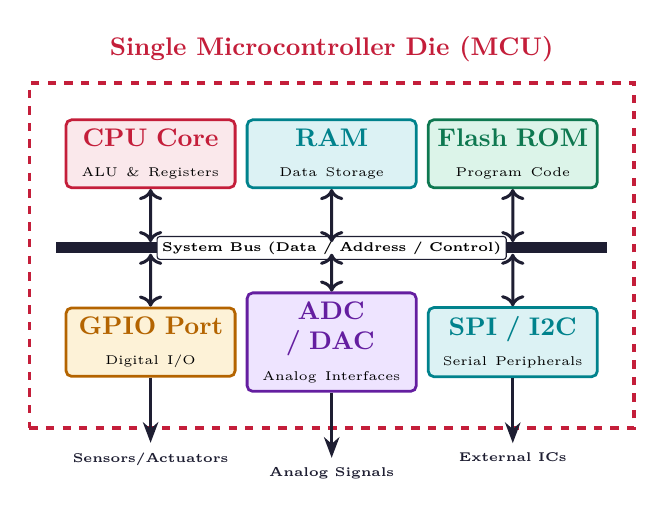
\begin{tikzpicture}[scale=0.92, transform shape]
  % System Bus (Central Backbone) - Label placed in center with white background to avoid boundary collision
  \draw[line width=4pt, color=mydark] (-3.8, 0) -- (3.8, 0);
  \node[font=\tiny\bfseries, fill=white, draw=mydark, rounded corners=1pt, inner sep=2pt] at (0,0) {System Bus (Data / Address / Control)};

  % Blocks above bus
  \node[draw=myred, fill=hdrred, rounded corners=2pt, line width=1pt, text width=2.1cm, align=center, minimum height=0.9cm] (cpu) at (-2.5, 1.3) {
    \textbf{\color{myred}CPU Core}\\
    \tiny ALU \& Registers
  };
  
  \node[draw=myteal, fill=hdrteal, rounded corners=2pt, line width=1pt, text width=2.1cm, align=center, minimum height=0.9cm] (ram) at (0, 1.3) {
    \textbf{\color{myteal}RAM}\\
    \tiny Data Storage
  };

  \node[draw=mygreen, fill=hdrgreen, rounded corners=2pt, line width=1pt, text width=2.1cm, align=center, minimum height=0.9cm] (flash) at (2.5, 1.3) {
    \textbf{\color{mygreen}Flash ROM}\\
    \tiny Program Code
  };

  % Blocks below bus
  \node[draw=myamber, fill=hdramber, rounded corners=2pt, line width=1pt, text width=2.1cm, align=center, minimum height=0.9cm] (gpio) at (-2.5, -1.3) {
    \textbf{\color{myamber}GPIO Port}\\
    \tiny Digital I/O
  };

  \node[draw=mypurple, fill=hdrpurple, rounded corners=2pt, line width=1pt, text width=2.1cm, align=center, minimum height=0.9cm] (adc) at (0, -1.3) {
    \textbf{\color{mypurple}ADC / DAC}\\
    \tiny Analog Interfaces
  };

  \node[draw=myteal, fill=hdrteal, rounded corners=2pt, line width=1pt, text width=2.1cm, align=center, minimum height=0.9cm] (serial) at (2.5, -1.3) {
    \textbf{\color{myteal}SPI / I2C}\\
    \tiny Serial Peripherals
  };

  % Bus taps (arrows)
  \draw[arrow, <->, line width=1.1pt] (cpu) -- (cpu |- 0, 0.08);
  \draw[arrow, <->, line width=1.1pt] (ram) -- (ram |- 0, 0.08);
  \draw[arrow, <->, line width=1.1pt] (flash) -- (flash |- 0, 0.08);
  \draw[arrow, <->, line width=1.1pt] (gpio) -- (gpio |- 0, -0.08);
  \draw[arrow, <->, line width=1.1pt] (adc) -- (adc |- 0, -0.08);
  \draw[arrow, <->, line width=1.1pt] (serial) -- (serial |- 0, -0.08);

  % Boundary Box (MCU Die)
  \node[draw=myred, dashed, line width=1.2pt, fit=(cpu) (ram) (flash) (gpio) (adc) (serial), inner sep=0.45cm] (mcu) {};
  \node[above=0.15cm of mcu, font=\bfseries\color{myred}] {Single Microcontroller Die (MCU)};
  
  % External interfaces - Lengthened arrows to Y=-2.8 to clear dashed boundary
  \draw[arrow, line width=1pt] (gpio.south) -- ++(0, -0.9) node[below, font=\tiny\bfseries] {Sensors/Actuators};
  \draw[arrow, line width=1pt] (adc.south) -- ++(0, -0.9) node[below, font=\tiny\bfseries] {Analog Signals};
  \draw[arrow, line width=1pt] (serial.south) -- ++(0, -0.9) node[below, font=\tiny\bfseries] {External ICs};
\end{tikzpicture}
\end{tcolorbox}

\subsection{Hardware Platforms Overview}
\begin{enumerate}[leftmargin=*, itemsep=4.0pt]
  \item \textbf{Arduino (Microcontroller-Based):} 
        \begin{itemize}[leftmargin=*, label=$\bullet$, itemsep=1.5pt]
          \item Powered by the \textbf{ATmega328P} 8-bit MCU operating at $16\text{ MHz}$, containing $32\text{ KB}$ Flash, $2\text{ KB}$ SRAM, and $1\text{ KB}$ EEPROM.
          \item Programmed in C++ using bare-metal register manipulation (e.g. setting \texttt{DDRB |= (1 << 5)} to configure Pin 13 as output, and writing to \texttt{PORTB} to toggle pins) compiled via \texttt{avr-gcc}.
          \item Ideal for low-power sleep modes ($<15\ \mu\text{A}$ in power-down mode) and deterministic, timing-critical sensor polling.
        \end{itemize}
  \item \textbf{Raspberry Pi (Single-Board Computer):}
        \begin{itemize}[leftmargin=*, label=$\bullet$, itemsep=1.5pt]
          \item Powered by a Broadcom \textbf{System-on-Chip (SoC)} containing a quad-core 64-bit ARM Cortex processor, up to $8\text{ GB}$ RAM, and GPU.
          \item Runs a fully pre-emptive Linux OS (Raspberry Pi OS) from an SD card. This introduces OS scheduling latency (non-deterministic) but allows full network stacks, file systems, and high-level runtimes (Python, Node.js).
          \item Used as local edge gateways, database hosts, and for CPU-intensive tasks like computer vision or edge AI inference.
        \end{itemize}
  \item \textbf{BeagleBone Black (PRU Co-processors):}
        \begin{itemize}[leftmargin=*, label=$\bullet$, itemsep=1.5pt]
          \item Features a $1\text{ GHz}$ ARM Cortex-A8 processor running Linux, augmented with two auxiliary \textbf{PRUs (Programmable Real-Time Units)}.
          \item Each PRU is a 32-bit RISC core operating at $200\text{ MHz}$ with direct access to hardware I/O pins and shared RAM, operating independently of the Linux kernel's interrupts or process schedules.
          \item Solves the "non-deterministic OS" issue, enabling sub-microsecond GPIO toggling, precise high-speed industrial motor control, and custom hardware protocol decoding.
        \end{itemize}
  \item \textbf{Electric Imp (Cloud-Integrated Module):}
        \begin{itemize}[leftmargin=*, label=$\bullet$, itemsep=1.5pt]
          \item A secure hardware module featuring an ARM Cortex processor and Wi-Fi interface.
          \item Utilizes a \textbf{Cloud-Device Split Model}: Code is split into a local \textit{Device} script (interfacing with pins) and a cloud-based \textit{Agent} script (running in Electric Imp's secure VM, handling HTTPS/OAuth).
          \item Programmed in the \textbf{Squirrel} scripting language. Features built-in secure boot, automated secure OTA firmware updates, and managed cloud routing.
        \end{itemize}
  \item \textbf{Mobile Phone and Tablets (Sensors \& Application Runtimes):}
        \begin{itemize}[leftmargin=*, label=$\bullet$, itemsep=1.5pt]
          \item High-performance mobile devices equipped with gigabytes of RAM, multi-core CPUs, and multi-Gbps cellular/Wi-Fi/Bluetooth networking.
          \item Host rich integrated sensors (dual-frequency GPS, 3-axis accelerometers, gyroscopes, magnetometers, ambient light sensors, cameras, and microphones).
          \item Used for rapid application-level prototyping, mobile dashboard display, and utilizing internal sensors as edge input devices.
        \end{itemize}
  \item \textbf{Plug Computing (Always-On Mini-Servers):}
        \begin{itemize}[leftmargin=*, label=$\bullet$, itemsep=1.5pt]
          \item Compact, wall-plug-sized, always-on servers containing a low-power MPU (e.g. Marvell Kirkwood ARM), RAM, flash storage, and an Ethernet/Wi-Fi connection.
          \item Run headless Linux server distributions (e.g., Debian).
          \item Act as quiet, unobtrusive, low-power local gateways, print servers, and local home automation hub controllers.
        \end{itemize}
\end{enumerate}

\newpage

% ═══════════════════════════════════════════════════════════════════════════════
% QUICK REVISION PAGE
% ═══════════════════════════════════════════════════════════════════════════════
\begin{center}
  {\large\bfseries\color{myred} Quick Revision — Module 3}\\[3pt]
  {\small\color{mydark} Embedded Hardware Platforms $|$ OE-EC803A}
\end{center}
\noindent{\color{myred}\rule{\linewidth}{1.2pt}}
\vspace{8pt}

\begin{tcolorbox}[formulabox, title={\textbf{Key Formulas and Metrics at a Glance}}]
\renewcommand{\arraystretch}{1.35}
\begin{tabularx}{\linewidth}{B{5.0cm} X}
  Ohm's Law & $V = I \cdot R \quad (\text{Volts, Amperes, Ohms})$ \\[4pt]
  Power dissipation & $P = V \cdot I = I^2 \cdot R \quad (\text{Watts})$ \\[4pt]
  PWM Effective Voltage & $V_{\text{eff}} = D \cdot V_{\text{max}} \quad (D = \text{Duty Cycle } \in [0, 1])$ \\[4pt]
  ADC Resolution & $V_{\text{step}} = \dfrac{V_{\text{ref}}}{2^N - 1} \quad (N\text{-bit Analog-to-Digital Converter})$
\end{tabularx}
\end{tcolorbox}

\vspace{6pt}

\begin{tcolorbox}[defbox, title={\textbf{One-Line Definitions}}]
\begin{itemize}[leftmargin=*, itemsep=3pt, topsep=0pt]
  \item \textbf{Microcontroller:} An IC integrating CPU, memory, and peripheral interfaces on a single chip.
  \item \textbf{Single-Board Computer:} A complete computer built on a single circuit board, running an operating system.
  \item \textbf{PRU (BeagleBone):} Co-processors that run independently of the main OS to execute real-time I/O tasks.
  \item \textbf{PWM:} A technique to simulate analog voltages by pulsing a digital output at varying widths.
  \item \textbf{Relay:} An electromechanical switch used to control high-power circuits with low-power digital signals.
\end{itemize}
\end{tcolorbox}

\vspace{6pt}

\begin{tcolorbox}[exambox, title={\textbf{Frequently Asked / Viva Questions}}]
\begin{enumerate}[leftmargin=*, topsep=0pt, label=\textbf{Q\arabic*.}, itemsep=6pt]
  \item \Q{What is the difference between a microcontroller and a microprocessor?}
        A microcontroller integrates the CPU, RAM, Flash memory, and I/O peripherals on a single silicon chip (System-on-Chip). A microprocessor contains only the CPU core and requires external components (RAM, Storage, Ethernet ICs) to function.
        
  \item \Q{Why are microcontrollers preferred over microprocessors for simple IoT sensor nodes?}
        Microcontrollers consume far less power (milliwatts vs. watts), support deep sleep modes that allow battery operation for years, are much cheaper, and run code directly on bare-metal without the boot latency of an operating system.
        
  \item \Q{What are the PRUs in a BeagleBone Black, and why are they useful?}
        The Programmable Real-Time Units (PRUs) are two auxiliary 32-bit RISC cores running at 200MHz independently of the main Linux OS. They allow BBB to perform fast, deterministic real-time I/O tasks without scheduling delays caused by the Linux kernel.
        
  \item \Q{Explain the concept of PWM and how it is used to dim an LED.}
        PWM (Pulse Width Modulation) switches a digital pin between high ($5\text{V}$) and low ($0\text{V}$) states rapidly. By changing the Duty Cycle (the fraction of time the pin is high), the effective average voltage varies continuously. This average voltage controls the LED brightness.
        
  \item \Q{What is a Single-Board Computer (SBC)? Give an example.}
        A Single-Board Computer is a complete, functioning computer built on a single circuit board, incorporating a microprocessor, memory, networking, and USB ports. An example is the Raspberry Pi, which runs a Debian-based Linux OS.
        
  \item \Q{How does a relay isolate a microcontroller from high-voltage appliances?}
        A relay uses an electromagnet. When the microcontroller energizes the internal coil (isolated low-voltage side), the magnetic field pulls a mechanical contact switch closed on the high-voltage side. There is no electrical connection between the two sides.
        
  \item \Q{Why is community support considered an important parameter when choosing prototyping hardware?}
        IoT development moves fast. A large active community ensures open-source driver libraries are available for almost any sensor, troubleshooting forum threads exist for common bugs, and development boards are widely stocked.
        
  \item \Q{What is Electric Imp, and how does it handle programming?}
        Electric Imp is a secure IoT module integrating Wi-Fi hardware with a managed cloud. It is programmed in the Squirrel scripting language, allowing developers to write both local device code and cloud agent code in a single framework.
\end{enumerate}
\end{tcolorbox}

\vspace{6pt}

\begin{tcolorbox}[tikzbox, title={\textbf{Comparison Snapshot}}]
\textbf{Arduino vs. Raspberry Pi vs. BeagleBone Black:}\par\vspace{6pt}\noindent
{\renewcommand{\arraystretch}{1.35}%
\begin{tabularx}{\linewidth}{|B{3.2cm}|Y|Y|Y|}
\hline
\textbf{Feature} & \textbf{Arduino Uno} & \textbf{Raspberry Pi 4} & \textbf{BeagleBone Black} \\
\hline
Type & Microcontroller (MCU) & Single-Board Computer (SBC) & Industrial SBC \\
\hline
Processor & 8-bit ATmega328P (16MHz) & 64-bit Quad ARM (1.5GHz) & 32-bit ARM (1GHz) + 2x PRUs \\
\hline
Memory & 2 KB SRAM, 32 KB Flash & 2GB / 4GB / 8GB LPDDR4 & 512MB DDR3, 4GB eMMC \\
\hline
Operating System & None (Bare-Metal) & Yes (Linux / Raspberry Pi OS) & Yes (Debian Linux) \\
\hline
Power Draw & Very Low (~50mW) & Medium-High (~3W to 5W) & Medium (~1.5W to 2.5W) \\
\hline
Best Use Case & Analog sensor read, relays. & Computer vision, IoT gateway. & Real-time industrial automation. \\
\hline
\end{tabularx}}
\end{tcolorbox}

\end{document}
